\documentclass[laboratorio]{guia}

\def \practnum {6} 
\def \practica {Ondas en una cuerda}
% \def \practica {Ondas estacionarias en una cuerda}

\def \materia {Laboratorio de F\'\i sica II para Qu\'\i micos}
\def \periodo {2do. Cuatrimestre de 2015}
\def \catedra {Pablo Cobelli}
\def \website {http://materias.df.uba.ar/f2qa2015c2}
 
\usepackage{graphics}
\usepackage{amsmath}
\usepackage{amsfonts}
\usepackage{graphicx}
\usepackage{float}
\usepackage{wrapfig}
\usepackage{subfigure}
\usepackage{bm}
\usepackage{grffile}
\usepackage{color}
\usepackage{framed}
\usepackage[utf8]{inputenc}
\usepackage[T1]{fontenc}
\usepackage{lmodern}
\usepackage{circuitikz}
\usepackage[spanish]{babel}
\usepackage{babelbib}
\selectbiblanguage{spanish}

 

%----------------------------------------------------------
% Agrega al path de figuras el subdirectorio con el mismo
%     nombre que el archivo principal del proyecto
\graphicspath{{./\jobname/}}

%----------------------------------------------------------
% Definicion del entorno 'sabermas'
\makeatletter
\definecolor{shadecolor}{rgb}{0.89,0.91,0.94}
\newenvironment{sabermas}[1]{%
\vfill
\begin{shaded}
  \begin{center}
  {\textsection{Para saber m\'as}}
  \end{center}
  #1
\sf } 
{%
\end{shaded}%
}
\makeatother

%----------------------------------------------------------
% Definicion del entorno 'problema'
\newcounter{ContadorProblema}
\setcounter{ContadorProblema}{0}
\newcounter{TieneFiguraAsociada}
\setcounter{TieneFiguraAsociada}{0}
\newcounter{UbicacionFigura}
\setcounter{UbicacionFigura}{0}

\newenvironment{problema}[2][]
{%
    \ifx\relax#1\relax%
        \setcounter{TieneFiguraAsociada}{0}
        \else
        \setcounter{TieneFiguraAsociada}{1}
    \fi
    \def \archivofigura {#1}
    % 
    \refstepcounter{ContadorProblema}
    \noindent%
    \ifnum\value{TieneFiguraAsociada} < 1%
        {\sffamily \bfseries Problema \arabic{ContadorProblema}.}
        %{\sc {#1}}%
        \par\nobreak\par\nobreak%
        \medskip 
    \else
        % Va con figura; resta determinar de que lado.
        \ifnum\value{UbicacionFigura} < 1
            % Poner la figura del lado derecho
            \begin{minipage}{12.25cm}
            {\sffamily \bfseries Problema \arabic{ContadorProblema}.}
            %{\sc {#1}}%
            \par\nobreak\par\nobreak%
            \medskip 
        \else
            % Poner la figura del lado izquierdo
            \begin{minipage}{4.5cm}
                \centering
                \includegraphics[width=4.5cm]{\archivofigura}
                {\footnotesize {\sffamily Esquema asociado al 
                problema \arabic{ContadorProblema}}.}
            \end{minipage}\hfill%
            \begin{minipage}{12.25cm}
                {\sffamily \bfseries Problema \arabic{ContadorProblema}.}
                %{\sc {#1}}%
                \par\nobreak\par\nobreak%
                \medskip 
        \fi
    \fi
}
{%
    \ifnum\value{TieneFiguraAsociada} < 1%
        % \par \bigskip \vskip 0.3cm
    \else
        % Va con figura; resta determinar de que lado.
        \ifnum\value{UbicacionFigura} < 1
            % Poner la figura del lado derecho
            \end{minipage}\hfill%
            \begin{minipage}{4.5cm}
                \centering
                \includegraphics[width=4.5cm]{\archivofigura}
                {\footnotesize {\sffamily Esquema asociado al 
                problema \arabic{ContadorProblema}}.}
            \end{minipage}
        \else
            % Poner la figura del lado izquierdo
            \end{minipage}%
        \fi
    \fi
    \setcounter{TieneFiguraAsociada}{0}
    \par \bigskip \vskip 0.3cm
    % Permutamos el valor de la ubicacion
    \ifnum\value{UbicacionFigura} < 1
        \setcounter{UbicacionFigura}{1}
    \else
        \setcounter{UbicacionFigura}{0}
    \fi
}

%----------------------------------------------------------
% Definicion/Redefinicion de estilos
\renewcommand{\vec}[1]{\ensuremath{\mathbf{#1}}}



\hyphenation{ coe-fi-cien-tes coe-fi-cien-te au-to-va-lor
              au-to-va-lo-res co-rres-pon-der pro-ble-ma 
              cual-quie-ra po-la-ri-za-cio-nes }

\graphicspath{{./cuerda/}}

\begin{document} 
\objetivo{
  Realizar un estudio experimental de ondas estacionarias en cuerdas con sus dos extremos fijos.
  Se propone medir los modos normales de vibración, determinando experimentalmente sus frecuencias características.
  En función de estos resultados, se busca determinar la velocidad de las ondas en términos de la tensión y la densidad de masa de la cuerda.
  \tematicas{ondas estacionarias, ondas en una cuerda, modos normales, frecuencias características, velocidad de propagación.}
} 
\maketitle


\section{Consideraciones preliminares}
La figura \ref{fig:1} muestra un esquema del dispositivo experimental propuesto para el desarrollo de esta experiencia.
\begin{figure}[htb]
    \centering
    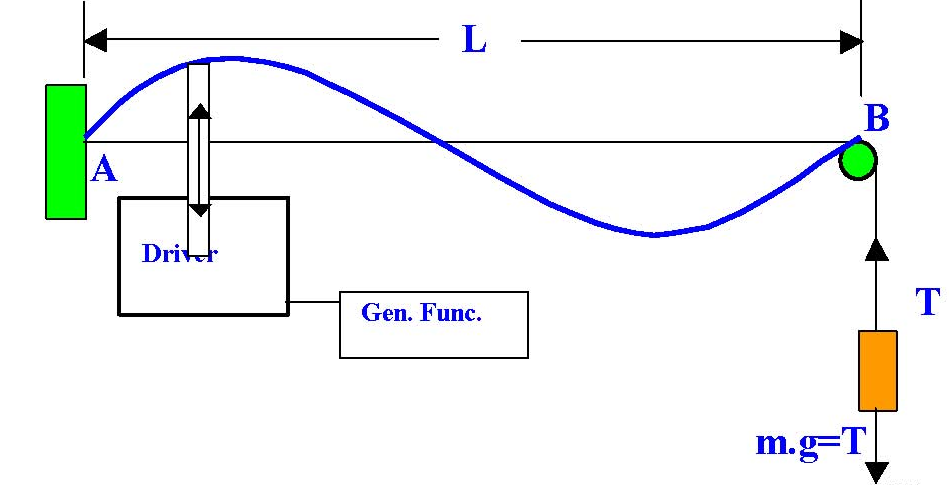
\includegraphics[width=8.5cm]{LG07--004.png}
    \caption{Esquema del montaje experimental propuesto para la realización de esta práctica.}
    \label{fig:1}
\end{figure}

En el mismo puede verse una cuerda (en trazo azul grueso) sujeta en sus dos extremos.
El extremo izquierdo está fijo a una pared (punto A), mientras que el extremo derecho está fijo a una polea (punto B).
La distancia entre los puntos A y B es \(L\).
Vinculado mecánicamente con la cuerda, más allá de la polea, se encuentra un objeto de masa \(m\), en reposo debido a la acción combinada de la gravedad y la tensión provista por la cuerda.
Cerca del punto A, un \textit{driver} mecánico imprime a la cuerda un movimiento oscilatorio armónico de frecuencia y amplitud controladas, provisto por un amplificador alimentando por un generador de funciones.
Utilizará un osciloscopio tanto para muestrear la frecuencia de la señal del generador como para verificar que a la entrada del \textit{driver} (conectores banana) la señal amplificada no supere los \SI{6}{\volt} pico a pico.

Para llevar a cabo la experiencia se dispone de una cuerda cuya masa por unidad de longitud \(\mu\) debe determinar experimentalmente a partir de la medición de la masa \(m_c\) del tramo de cuerda que haya cortado para utilizar.
La tensión mecánica que actúa sobre la cuerda está determinada por el peso colgado en uno de sus extremos, según se observa en la figura \ref{fig:1}. 

La longitud de onda de cada modo excitado por el \textit{driver} está determinada por la longitud de la cuerda, ya que la longitud \(L\) es siempre igual a un número entero de veces media longitud de onda.

Antes de continuar, asegúrese de poder responder estas dos preguntas:
\begin{itemize}
    \item ¿Por qué vale \(L = (n+\frac{1}{2}) \lambda\), siendo \(n \in \mathbb{N}_0\) entero? 
    \item ¿Cómo haría para conocer \(\mu\) en sus condiciones de trabajo?
\end{itemize}



\section{Desarrollo de la experiencia}

\subsection{Velocidad de propagación en un modo}
Mida las frecuencias \(f_i\) y longitud de onda correspondiente \(\lambda_i\), que se corresponden con una única \(m\) en el plantillo, para los primeros modos.
Si suponemos que la velocidad es la misma para todos los primeros \(n\) modos, debe verificarse en todos los casos que
\begin{equation}
  v= \lambda_n f_n,
  \label{eq:erste}
\end{equation}
así que si se obtiene el logaritmo el logaritmo de esta expresión queda
\begin{equation}
  \log{v}= \log{\left(\lambda_n f_n \right)}= \log{\lambda_n}+ \log{f_n}.
  \label{eq:zweite}
\end{equation}
Con la expresión (\ref{eq:zweite}) basta graficar un logaritmo en función del otro y obtener, a través del ajuste de una función lineal, la ordenada al origen para de esta obtener \(v\).
No olvide que debe elegir como parámetro dependiente aquél logaritmo que presente el mayor error relativo en vistas a la evaluación del error del ajuste por el método de cuadrados mínimos.



\subsection{Distintas velocidades de propagación}
Recordemos que la velocidad de la onda en una cuerda depende de la tensión a la que se la somete, y por tanto de la masa en el platillo \(m_i\) (pesas mas platillo en sí)
\begin{equation}
  v_i= \sqrt{\frac{T_i}{\mu}}= \sqrt{\frac{g m_i}{\mu}}.
\end{equation}
Lo que se propone es que manteniendo el mismo modo, es decir, en el que observará la misma \(\lambda_n\) al variar \(m_i\) registre cada frecuencia \(f_i\) y con ellas obtenga una gráfica de \(v_i\) en función de cada \(T_i\).
No olvide que \(m_i\) incluye no solo comprente la masa aportada por las pesas sino también la del platillo.
¿Que conclusión obtiene?


\subsection{Constante elástica de la cuerda}
En el ejercicio anterior se hizo una suposición muy fuerte de que no importa a que \(T_i\) se sometiera la cuerda, la \(\mu\) de esta no variaba, es decir que \emph{la cuerda no se estira}.
La cuerda que utiliza está fabricada a partir de un polímero.
La unión entre monómeros presenta un régimen elástico hasta cierta \(T_i\) y luego uno plástico.

Se propone explorar el primero utilizando valores moderados de \(m_i\) que supondremos se relacionan con distintas longitudes de la cuerda \(L_i\).
Modelando un estiramiento elástico proporcional a una constante \(k\), cada \(L_i\) que supere a una longitud de referencia \(L_o\) que se alcanza con una \(T_o= m_o g\) será causada por una \(m_i > m_o\).
Así \(L_i= L_o+ k (m_i - m_o) g\) y la nueva relación entre la velocidad de la onda y y la masa colgada \(m_i\) quedaría modelada por
\begin{equation}
  v_i = \lambda_n f_i= \sqrt{\frac{m_i g}{m_c}\left[L_o + k (m_i - m_o) g \right] },
  \label{eq:1}
\end{equation}
siendo \(m_c\) es la masa total de la cuerda.
Un poco de álgebra permite llegar a que
\begin{equation}
  f_i^2 = \frac{k g^2}{m_c \lambda_n^2} m_i^2+ \frac{g}{m_c \lambda_n^2} \left(L_o- k m_o g \right) m_i,
  \label{eq:2}
\end{equation}

Cada vez que varíe \(m_i\) modifique también \(f_i\) a fin de reproducir \emph{siempre} la misma \(\lambda_n\).
Determine las dos estimaciones del \(k\) que arrojan un ajuste de la función \ref{eq:2} a las mediciones así realizadas.



\nocite{Alonso1998,Crawford1994}
\bibliographystyle{unsrt} 
\bibliography{Bibliografia}


\end{document}
